\documentclass[12pt]{article}
\usepackage[top=1in,bottom=1in,left=1in,right=1in]{geometry}
\usepackage{alltt}
\usepackage{array}	
\usepackage{graphicx}
\usepackage{tabularx}
\usepackage{verbatim}
\usepackage{setspace}
\usepackage{listings}
\usepackage{amssymb,amsmath, amsthm}
\usepackage{qtree}
\usepackage{hyperref}
\usepackage{oz}
\usepackage[cc]{titlepic}
\usepackage{fancyvrb}
\usepackage{epstopdf}

\title{SOEN 331 (Section): Introduction to Formal Methods\\for Software Engineering\\
\ \\
Assignment 3 on Temporal Logic}
\author{\begin{tabular}{c}
Alec Adub (40032876) - \texttt{adub.alec@gmail.com} \tabularnewline
Alex Frappier Lachapelle (40019133) - \texttt{alexfl1024@gmail.com} \tabularnewline
Robert Nittolo (40032587) - \texttt{nittolorobert@yahoo.com} \tabularnewline
Pierre-Olivier Trottier (40059235) - \texttt{po.trottier@gmail.com} \tabularnewline\\
\end{tabular}
}
\date{\today}
\begin{spacing}{1.5}
\begin{document}
\maketitle

\newpage

\section*{Problem 1 (20 pts):  Analyzing program behavior}

\begin{enumerate}

\item (10 pts) Visualize all models of behavior.

\begin{figure}[h!]
  \centering
  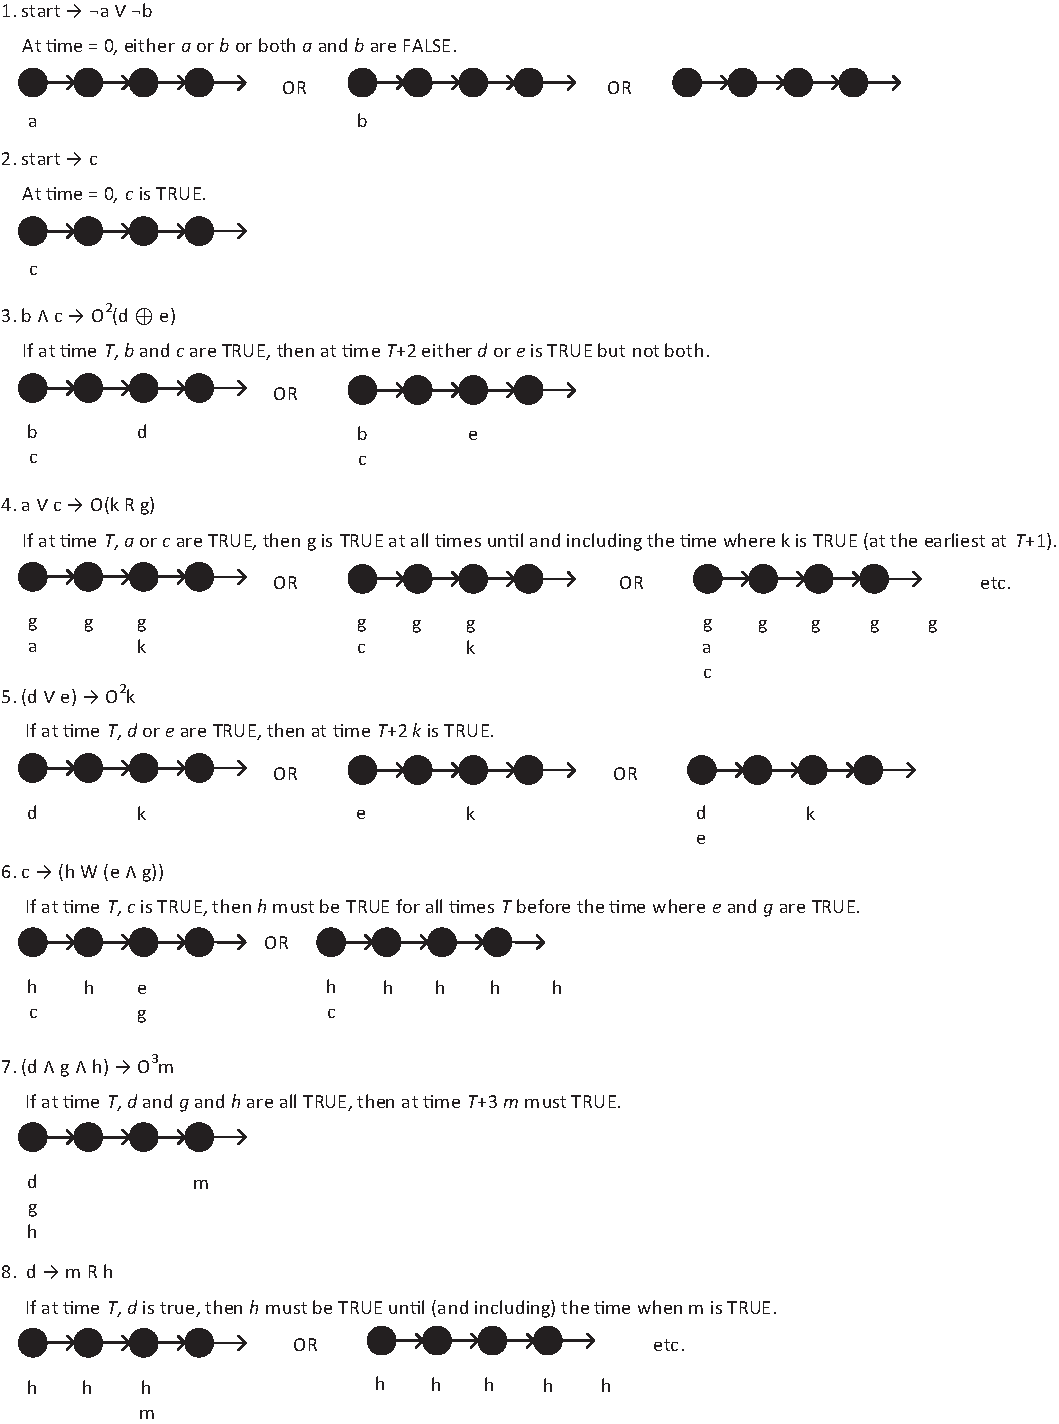
\includegraphics[width=0.9\textwidth]{q1-part1.pdf}
\end{figure}

\newpage

\begin{figure}[h!]
  \centering
  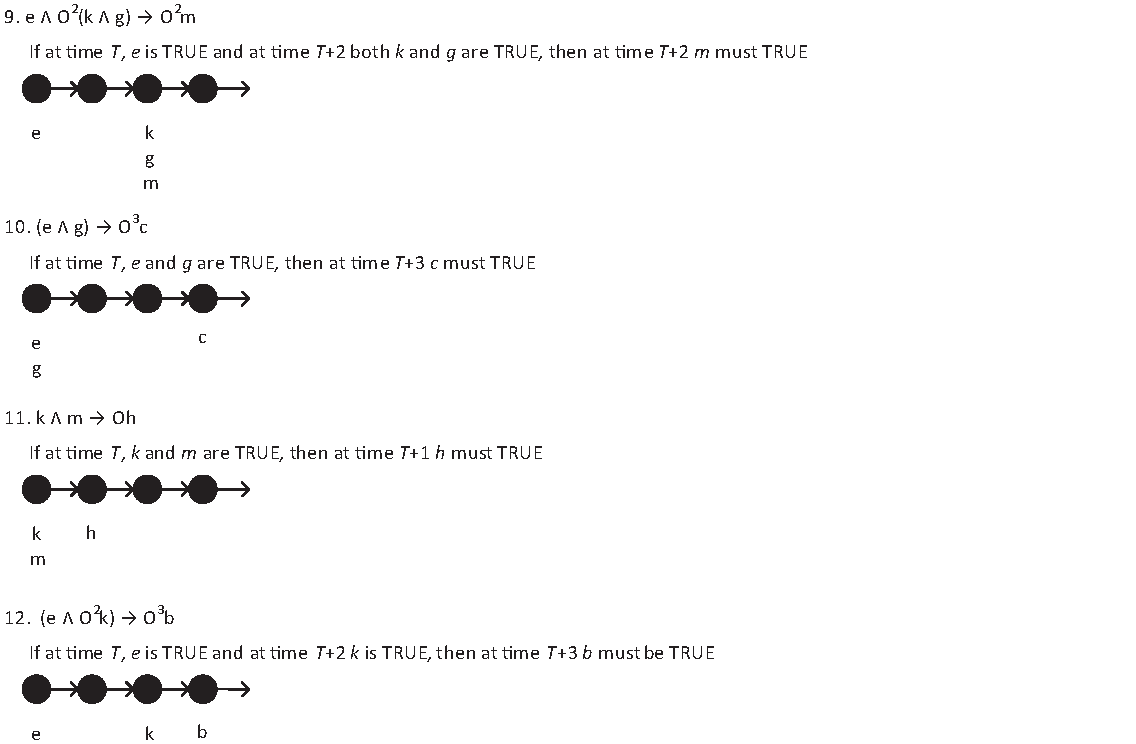
\includegraphics[width=0.9\textwidth]{q1-part2.pdf}
\end{figure}

\item (3 pts) Specify conditions (model of behavior), if any exist, under which the program can terminate.
\\
Conditions do exist for the program to terminate 

1)
$\langle(a\vee c),g,gk\rangle.$	
\\
2)
$\langle(b\wedge c),e,k,b\rangle.$	



\item (7 pts) For the expressions below, indicate (true/false) whether there exists a 
model where the expression holds. When true, cross reference your particular model:

\begin{table}\small
\centering
\begin{tabular}{|l|l|}
\hline
\textbf{PROPERTY}							& \textbf{TRUE/FALSE}\\
\hline

$(a \wedge c) \rightarrow \Diamond \Box (g \wedge h)$	
 &\textbf{TRUE}\\
 &\textbf{Crossreferemced with behavior 6}\\
&\\

\hline


		
$h ~\mathcal{U}~ m$									 
 &\textbf{TRUE}\\
 &\textbf{Crossreferemced with behavior 5}\\
&\\

\hline

&\\
		
$h ~\mathcal{U}~ (k \wedge g)$						
 &\textbf{FALSE}\\

&\\

\hline

&\\
		
$(b \wedge c) \rightarrow \Box \Diamond (b \wedge c)$ 
 &\textbf{FALSE}\\
&\\

\hline

&\\
		
$(k \wedge \bigcirc (k \wedge g)) \rightarrow \bigcirc m$ 
 &\textbf{FALSE}\\
&\\

\hline

&\\
		
$ h ~\mathcal{S}~ c$							
 &\textbf{TRUE}\\
 &\textbf{Crossreferemced with behavior 6}\\
&\\

\hline

&\\
		
$ ((g \wedge h) \wedge \bigcirc d) \rightarrow \bigcirc^{2} (g \wedge h)$
 &\textbf{FALSE}\\
&\\

\hline

&\\
		
$e ~\mathcal{R}~ h$								
 &\textbf{TRUE}\\
 &\textbf{Crossreferemced with behavior 8}\\
&\\

\hline

&\\
		
The program has the following stability property: &\\
$\Diamond \Box (b \wedge \ c \wedge h)$		
 &\textbf{FALSE}\\
&\\

\hline

&\\
		
The program has the following recurrence property: &\\
$\Box \Diamond (b \wedge \ c \wedge h)$		
 &\textbf{TRUE}\\
 &\textbf{Crossreferemced with behavior 9}\\
&\\

\hline

&\\
		
$( g \wedge h)$ is an invariant property of the program.  
 &\textbf{TRUE}\\
 &\textbf{Crossreferemced with behavior 8}\\
&\\

\hline

&\\
		
There is a guarantee that $(g \wedge k \wedge h)$	
 &\textbf{TRUE}\\
 &\textbf{Crossreferemced with behavior 9}\\
&\\

\hline

	
The program has the following property: &\\
$(b \wedge c \wedge h) \rightarrow \Diamond (b \wedge c \wedge h)$.   
 &\textbf{FALSE}\\


\hline

		
The program has the following precedence property: &\\
$(b \wedge c \wedge h) \rightarrow ( (g \wedge h) ~\mathcal{U}~ b \wedge c \wedge h))$
	 &\textbf{FALSE}\\	
&\\

\hline

\end{tabular}
\end{table}


\end{enumerate}


\newpage

\section*{Problem 2 (20 pts) :  Visualizing temporal expressions}

\begin{enumerate}

	\item $\Box (\phi \rightarrow \bigcirc^{2} \psi)$
	
	If $\phi$ is true at some moment, then $\psi$ is true at the next 		next moment.
	
	$\bullet-\bullet-\bullet-\bullet-\bullet-\bullet-\bullet$ \newline
	$\phi-\circ-\psi-\circ-\circ-\circ-\circ$ \newline
	or \newline
	$\bullet-\bullet-\bullet-\bullet-\bullet-\bullet-\bullet$ \newline
	$\circ-\circ-\circ-\circ-\phi-\circ-\psi$ \newline
	etc... 

	\item $\Box \phi \rightarrow \bigcirc \psi$
	
	If $\phi$ is globally true it implies that next $\psi$ is true.
	
	$\bullet-\bullet-\bullet-\bullet-\bullet-\bullet$ \newline
	$\phi-\phi-\phi-\phi-\phi-\phi$ \newline
	$\circ-\psi-\circ-\circ-\circ-\circ$
	
	\item $\phi \rightarrow \bigcirc \Diamond \Box \psi$
	
	$\phi$ implies $\psi$ becomes globally true at some point in time starting i+1.
	
	$\bullet-\bullet-\bullet-\bullet-\bullet-\bullet$ \newline
	$\phi-\psi-\psi-\psi-\psi-\psi$ \newline
	or \newline
	$\bullet-\bullet-\bullet-\bullet-\bullet-\bullet$ \newline
	$\phi-\circ-\circ-\psi-\psi-\psi$ \newline
	etc...
	
	\item $(\phi \wedge \bigcirc \psi) \rightarrow \bigcirc^{2} \Diamond \Box \omega$
	
	$\phi$ and next $\psi$ implies that $\omega$ becomes globally true at some point in time starting i+2.
	
	$\bullet-\bullet-\bullet-\bullet-\bullet-\bullet$ \newline
	$\phi-\psi-\omega-\omega-\omega-\omega$ \newline
	or \newline
	$\bullet-\bullet-\bullet-\bullet-\bullet-\bullet-\bullet$ \newline
	$\phi-\psi-\circ-\circ-\omega-\omega-\omega$ \newline
	etc...
	
	\item $\Box ((\phi \wedge \bigcirc \psi) \rightarrow \bigcirc^{2} \Diamond \Box \omega)$
	
	If $\phi$ and $\psi$ next is true at some moment, then $\omega$ becomes globally true at some point in time at the next next moment. 
	
	$\bullet-\bullet-\bullet-\bullet-\bullet-\bullet$ \newline
	$\phi-\psi-\omega-\omega-\omega-\omega$ \newline
	or \newline
	$\bullet-\bullet-\bullet-\bullet-\bullet-\bullet-\bullet$ \newline
	$\phi-\psi-\circ-\circ-\omega-\omega-\omega$ \newline
	or \newline
	$\bullet-\bullet-\bullet-\bullet-\bullet-\bullet$ \newline
	$\circ-\circ-\phi-\psi-\omega-\omega$ \newline
	etc...
	
	\item $(\phi \wedge \bigcirc \psi) \rightarrow \tau ~\mathcal{R}~ \upsilon$ \newline
	$\bullet-\bullet-\bullet-\bullet$ \newline
	$\phi-\psi-\circ-\circ$ \newline
	$\upsilon-\upsilon-\upsilon-\circ$ \newline
	$\circ-\circ-\tau-\circ$ \newline
	or \newline
	$\bullet-\bullet-\bullet-\bullet-\bullet-$ \newline
	$\phi-\psi-\circ-\circ-\circ$ \newline
	$\upsilon-\upsilon-\upsilon-\upsilon-\upsilon-\upsilon$ \newline
	etc...
	
	\item $(\phi \wedge \bigcirc \psi) \rightarrow \bigcirc (\tau ~\mathcal{R}~ \upsilon)$ \newline
	$\bullet-\bullet-\bullet-\bullet-\bullet$ \newline
	$\phi-\psi-\circ-\circ-\circ$ \newline
	$\circ-\upsilon-\upsilon-\upsilon-\circ$ \newline
	$\circ-\circ-\circ-\tau-\circ$ \newline
	or \newline
	$\bullet-\bullet-\bullet-\bullet-\bullet-$ \newline
	$\phi-\psi-\circ-\circ-\circ$ \newline
	$\circ-\upsilon-\upsilon-\upsilon-\upsilon-\upsilon$ \newline
	etc...

	\item $(\phi \wedge \bigcirc \psi) \rightarrow \bigcirc (x ~\mathcal{U}~ \tau)$ \newline
	$\bullet-\bullet-\bullet-\bullet-\bullet$ \newline
	$\phi-\psi-\circ-\circ-\circ$ \newline
	$\circ-x-x-\circ-\circ$ \newline
	$\circ-\circ-\circ-\tau-\circ$ \newline
	or \newline
	$\bullet-\bullet-\bullet-\bullet$ \newline
	$\phi-\psi-\circ-\circ$ \newline
	$\circ-x-\circ-\circ$ \newline
	$\circ-\circ-\tau-\circ$ \newline
	etc...
	
	\item $(\phi \wedge \Box \psi) \rightarrow \bigcirc^{2} \Diamond \omega$ \newline
	$\bullet-\bullet-\bullet-\bullet-$ \newline\
	$\phi-\circ-\circ-\circ$ \newline
	$\psi-\psi-\psi-\psi-\psi$\newline
	$\circ-\circ-\omega-\circ$\newline
	or \newline
	$\bullet-\bullet-\bullet-\bullet-$ \newline\
	$\phi-\circ-\circ-\circ$ \newline
	$\psi-\psi-\psi-\psi-\psi$\newline
	$\circ-\circ-\circ-\circ-\omega$\newline
	etc...
	
	
	\item $(\phi \wedge \bigcirc^{2} \psi) \rightarrow \bigcirc \Box \omega$ \newline
	$\bullet-\bullet-\bullet-\bullet-$ \newline\
	$\phi-\circ-\circ-\circ$ \newline
	$\circ-\circ-\psi-\circ$\newline
	$\circ-\omega-\omega-\omega-\omega$\newline


\end{enumerate}

\end{spacing}
\end{document}